\documentclass[aspectratio=169,11pt]{beamer}

\usepackage[T1]{fontenc}
\usepackage{lmodern}
\usepackage[ngerman]{babel}
\usepackage{booktabs}
\usepackage{array}
\usepackage{tikz}
\usepackage{pgfplots}
\pgfplotsset{compat=1.18}
\usetikzlibrary{babel}
\usepgfplotslibrary{fillbetween}

% --- Erscheinungsbild ---------------------------------------------------------
\definecolor{hkared}{RGB}{198, 42, 18}
\definecolor{tinte}{HTML}{22262B}
\definecolor{grautext}{HTML}{5C636B}
\definecolor{gitter}{HTML}{E5E4E0}
\definecolor{blau}{HTML}{2A78D6}
\definecolor{orange}{HTML}{EB6834}
\definecolor{gruen}{HTML}{0F8A5F}
\definecolor{flaeche}{HTML}{DCE9F8}

\setbeamertemplate{navigation symbols}{}
\setbeamertemplate{footline}{\hfill\color{grautext}\scriptsize\insertframenumber\,/\,\inserttotalframenumber\hspace{4mm}\vspace{2mm}}
\setbeamercolor{normal text}{fg=tinte,bg=white}
\setbeamercolor{frametitle}{fg=hkared,bg=white}
\setbeamercolor{title}{fg=hkared}
\setbeamercolor{subtitle}{fg=grautext}
\setbeamercolor{date}{fg=grautext}
\setbeamercolor{item}{fg=hkared}
\setbeamerfont{frametitle}{size=\Large,series=\bfseries}
\setbeamerfont{title}{size=\LARGE,series=\bfseries}
\setbeamertemplate{itemize items}[circle]
\setlength{\leftmargini}{1.2em}

\pgfplotsset{
  prachse/.style={
    width=7.2cm, height=5.6cm,
    xmin=0, xmax=1.05, ymin=0, ymax=1.05,
    xlabel={Recall}, ylabel={Precision},
    xtick={0,0.2,0.4,0.6,0.8,1}, ytick={0,0.2,0.4,0.6,0.8,1},
    /pgf/number format/use comma,
    grid=major, grid style={gitter},
    axis line style={grautext}, tick style={grautext},
    tick label style={font=\scriptsize, text=grautext},
    label style={font=\small, text=grautext},
    axis on top=false,
  }
}

\newcommand{\hl}[1]{\textbf{#1}}
\newcommand{\quelle}[1]{\par\vfill{\scriptsize\color{grautext}#1\par}}

\title{Die Precision-Recall-Kurve verstehen}
\subtitle{KI-Labor, Assignment 5: Fußgängererkennung mit Faster R-CNN (Penn-Fudan)}
\date{}

\begin{document}

% ------------------------------------------------------------------------------
\begin{frame}[plain]
  \titlepage
\end{frame}

% ------------------------------------------------------------------------------
\begin{frame}{Ein Detektor liefert Boxen mit einem Score}
  Für jede Box gibt das Modell an, wie sicher es sich ist: den \hl{Score} zwischen 0 und 1.
  Eine Box zählt als Treffer, wenn sie eine echte Person mit einer IoU von mindestens 0,5 überlappt.

  \vspace{5mm}
  \centering
  \renewcommand{\arraystretch}{1.35}
  \begin{tabular}{>{\bfseries}l l l}
    \toprule
    Abkürzung & Bedeutung & Fall im Bild \\
    \midrule
    {\color{gruen}TP} & True Positive & Box liegt richtig auf einer Person \\
    {\color{orange}FP} & False Positive & Box ohne passende Person: ein Fehlalarm \\
    {\color{blau}FN} & False Negative & Person ohne passende Box: verpasst \\
    \bottomrule
  \end{tabular}
\end{frame}

% ------------------------------------------------------------------------------
\begin{frame}{Precision und Recall stellen zwei verschiedene Fragen}
  \begin{columns}[T,onlytextwidth]
    \begin{column}{0.47\textwidth}
      \hl{Precision}\\[1mm]
      {\color{grautext}Wie viele Vorhersagen stimmen?}
      \[
        \text{Precision} = \frac{\text{TP}}{\text{TP} + \text{FP}}
      \]
      Niedrig bedeutet: viele Fehlalarme.
    \end{column}
    \begin{column}{0.47\textwidth}
      \hl{Recall}\\[1mm]
      {\color{grautext}Wie viele Personen wurden gefunden?}
      \[
        \text{Recall} = \frac{\text{TP}}{\text{TP} + \text{FN}}
      \]
      Niedrig bedeutet: viele verpasste Personen.
    \end{column}
  \end{columns}

  \vspace{7mm}
  Jeder Wert allein täuscht: Wer jede denkbare Box meldet, erreicht einen hohen Recall.
  Wer nur die eine sicherste Box meldet, erreicht leicht eine hohe Precision.
\end{frame}

% ------------------------------------------------------------------------------
\begin{frame}{Die Score-Schwelle regelt den Kompromiss}
  \begin{columns}[c,onlytextwidth]
    \begin{column}{0.54\textwidth}
      \centering
      \renewcommand{\arraystretch}{1.25}
      \begin{tabular}{c r r r}
        \toprule
        \textbf{Schwelle} & \textbf{FP} & \textbf{Precision} & \textbf{Recall} \\
        \midrule
        0,3 & 239 & 0,633 & 0,976 \\
        0,5 & 140 & 0,746 & 0,974 \\
        0,8 &  64 & 0,863 & 0,950 \\
        \bottomrule
      \end{tabular}

      \vspace{2mm}
      {\scriptsize\color{grautext}COCO-Modell, Klasse „person“, alle 170 Bilder}
    \end{column}
    \begin{column}{0.42\textwidth}
      \begin{itemize}
        \setlength{\itemsep}{3mm}
        \item \hl{Hohe Schwelle:} Das Modell meldet weniger. Die Precision steigt, der Recall sinkt.
        \item \hl{Niedrige Schwelle:} Das Modell meldet mehr. Der Recall steigt, die Precision sinkt meist.
      \end{itemize}
    \end{column}
  \end{columns}

  \vspace{6mm}
  Die Tabelle zeigt nur drei Schwellen. \hl{Die Kurve zeigt alle auf einmal.}
\end{frame}

% ------------------------------------------------------------------------------
\begin{frame}{So entsteht die Kurve: sortieren und mitzählen}
  \begin{columns}[c,onlytextwidth]
    \begin{column}{0.5\textwidth}
      \small
      \centering
      \renewcommand{\arraystretch}{1.08}
      \begin{tabular}{r c c c}
        \toprule
        \textbf{Score} & \textbf{Ergebnis} & \textbf{Precision} & \textbf{Recall} \\
        \midrule
        0,99 & {\color{gruen}\textbf{TP}} & $1/1 = 1{,}00$ & $1/5 = 0{,}2$ \\
        0,95 & {\color{gruen}\textbf{TP}} & $2/2 = 1{,}00$ & $2/5 = 0{,}4$ \\
        0,90 & {\color{orange}\textbf{FP}} & $2/3 = 0{,}67$ & $2/5 = 0{,}4$ \\
        0,80 & {\color{gruen}\textbf{TP}} & $3/4 = 0{,}75$ & $3/5 = 0{,}6$ \\
        0,70 & {\color{gruen}\textbf{TP}} & $4/5 = 0{,}80$ & $4/5 = 0{,}8$ \\
        0,60 & {\color{orange}\textbf{FP}} & $4/6 = 0{,}67$ & $4/5 = 0{,}8$ \\
        0,40 & {\color{gruen}\textbf{TP}} & $5/7 = 0{,}71$ & $5/5 = 1{,}0$ \\
        \bottomrule
      \end{tabular}

      \vspace{2mm}
      {\scriptsize\color{grautext}Erfundenes Rechenbeispiel mit 5 echten Personen}
    \end{column}
    \begin{column}{0.47\textwidth}
      \centering
      \begin{tikzpicture}
        \begin{axis}[prachse, width=6.8cm, height=5.5cm]
          \addplot[blau, thick, mark=*, mark size=1.8pt] coordinates {
            (0.2,1) (0.4,1) (0.4,0.667) (0.6,0.75) (0.8,0.8) (0.8,0.667) (1,0.714)
          };
        \end{axis}
      \end{tikzpicture}
    \end{column}
  \end{columns}

  \vspace{3mm}
  Die Vorhersagen sind nach Score sortiert, jede Zeile entspricht also einer niedrigeren Schwelle.
  Ein \textcolor{gruen}{\textbf{TP}} führt nach rechts, ein \textcolor{orange}{\textbf{FP}} senkrecht nach unten.
\end{frame}

% ------------------------------------------------------------------------------
\begin{frame}{Die Fläche unter der geglätteten Kurve ist die Average Precision}
  \begin{columns}[c,onlytextwidth]
    \begin{column}{0.47\textwidth}
      \centering
      \begin{tikzpicture}
        \begin{axis}[prachse, width=6.8cm, height=5.5cm]
          \addplot[draw=none, fill=flaeche, forget plot] coordinates {
            (0,0) (0,1) (0.4,1) (0.4,0.8) (0.8,0.8) (0.8,0.714) (1,0.714) (1,0)
          } \closedcycle;
          \addplot[grautext!60, thin, mark=*, mark size=1.2pt, forget plot] coordinates {
            (0.2,1) (0.4,1) (0.4,0.667) (0.6,0.75) (0.8,0.8) (0.8,0.667) (1,0.714)
          };
          \addplot[blau, very thick] coordinates {
            (0,1) (0.4,1) (0.4,0.8) (0.8,0.8) (0.8,0.714) (1,0.714)
          };
          \node[font=\small, text=tinte] at (axis cs:0.5,0.38) {AP $=$ Fläche};
        \end{axis}
      \end{tikzpicture}
    \end{column}
    \begin{column}{0.49\textwidth}
      \hl{Glätten:} Die graue Zickzacklinie wird zur blauen Treppe. Jeder Punkt übernimmt die beste Precision, die weiter rechts noch erreichbar ist.

      \vspace{4mm}
      \hl{Fläche ausrechnen:}
      \[
        0{,}4 \cdot 1{,}00 + 0{,}4 \cdot 0{,}80 + 0{,}2 \cdot 0{,}71 \approx 0{,}86
      \]

      \vspace{1mm}
      Die Average Precision fasst die ganze Kurve in einer Zahl zusammen.
      Genau das rechnet \texttt{average\_precision} im Notebook.
    \end{column}
  \end{columns}
\end{frame}

% ------------------------------------------------------------------------------
\begin{frame}{Beim Lesen zählen die Ecke oben rechts und der Arbeitspunkt}
  \begin{columns}[c,onlytextwidth]
    \begin{column}{0.5\textwidth}
      \centering
      \begin{tikzpicture}
        \begin{axis}[prachse, width=7.2cm, height=5.8cm, ymax=1.2]
          \addplot[blau, very thick, smooth] coordinates {
            (0,1) (0.5,0.99) (0.75,0.97) (0.88,0.92) (0.95,0.8) (1,0.55)
          };
          \addplot[orange, very thick, smooth] coordinates {
            (0,0.95) (0.25,0.85) (0.5,0.68) (0.7,0.5) (0.85,0.34) (0.95,0.2)
          };
          \addplot[only marks, mark=*, mark size=3.2pt, blau, mark options={draw=white, line width=0.8pt}] coordinates {(0.88,0.92)};
          \addplot[only marks, mark=o, mark size=2.8pt, tinte] coordinates {(1,1)};
          \draw[grautext, thin] (axis cs:0.86,0.89) -- (axis cs:0.80,0.74);
          \node[anchor=north, font=\footnotesize, text=tinte] at (axis cs:0.76,0.75) {Arbeitspunkt};
          \node[anchor=south, font=\footnotesize, text=tinte] at (axis cs:0.3,1.0) {starkes Modell};
          \node[anchor=north west, font=\footnotesize, text=tinte] at (axis cs:0.03,0.6) {schwaches Modell};
          \node[anchor=south east, font=\footnotesize, text=grautext] at (axis cs:1.03,1.03) {Ideal};
        \end{axis}
      \end{tikzpicture}

      {\scriptsize\color{grautext}Schematische Skizze, keine Messwerte}
    \end{column}
    \begin{column}{0.46\textwidth}
      \begin{itemize}
        \setlength{\itemsep}{2.5mm}
        \item \hl{Weiter oben rechts ist besser.} Das Modell findet viele Personen und macht dabei wenige Fehler.
        \item \hl{Ein spätes Abfallen ist gut.} Die Precision bleibt dann auch bei hohem Recall hoch.
        \item \hl{Der Arbeitspunkt} ist die Stelle, die eine konkrete Schwelle auf der Kurve auswählt.
        \item \hl{Die Anwendung entscheidet,} welche Stelle die richtige ist.
      \end{itemize}
    \end{column}
  \end{columns}
\end{frame}

% ------------------------------------------------------------------------------
\begin{frame}{In unserem Versuch sind alle drei Modelle sehr gut}
  \centering
  \makebox[\textwidth][c]{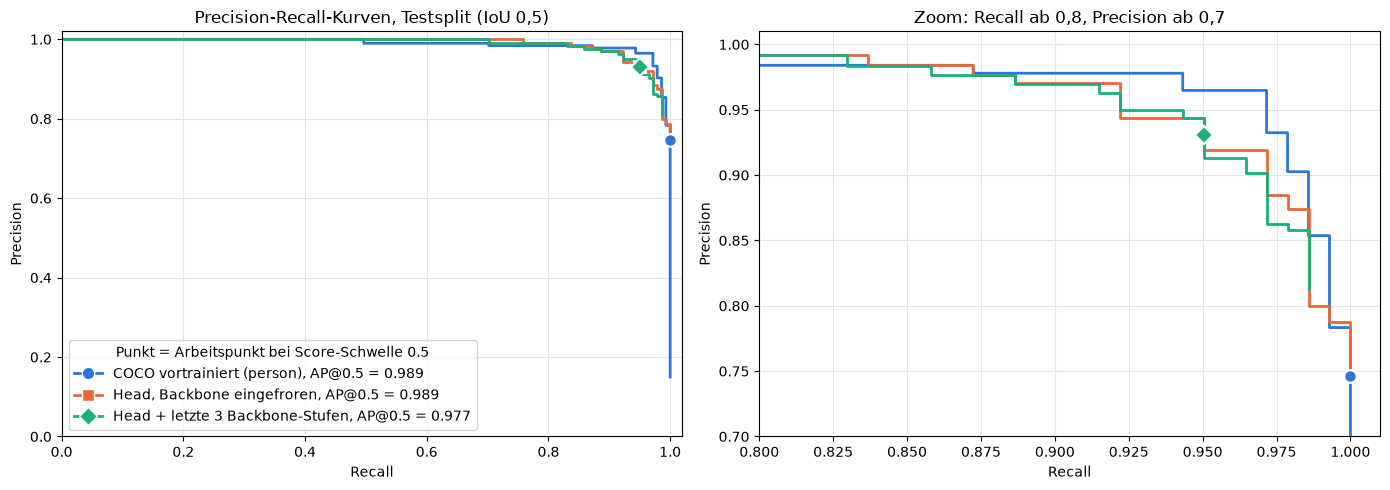
\includegraphics[width=15.4cm]{pr_kurven_notebook.png}}

  \vspace{1mm}
  \raggedright
  Bis zu einem Recall von etwa 0,9 bleibt die Precision bei allen über 0,94. Unterschiede gibt es fast nur danach.
  \quelle{Testsplit: 50 Bilder, 141 Personen, IoU 0,5. Abbildung aus Abschnitt 8 des Notebooks.}
\end{frame}

% ------------------------------------------------------------------------------
\begin{frame}{Gleiche AP, aber verschiedene Arbeitspunkte}
  \centering
  \renewcommand{\arraystretch}{1.3}
  \begin{tabular}{l r r r}
    \toprule
    \textbf{Modell} & \textbf{AP@0,5} & \textbf{Recall} & \textbf{Precision} \\
    \midrule
    COCO vortrainiert (person) & 0,989 & 1,000 & 0,746 \\
    Head, Backbone eingefroren & 0,989 & 0,950 & 0,931 \\
    Head + letzte 3 Backbone-Stufen & 0,977 & 0,950 & 0,931 \\
    \bottomrule
  \end{tabular}

  \vspace{1mm}
  {\scriptsize\color{grautext}Recall und Precision bei Score-Schwelle 0,5, gleicher Lauf wie die Abbildung}

  \vspace{6mm}
  \raggedright
  \begin{itemize}
    \setlength{\itemsep}{2.5mm}
    \item Das COCO-Modell und das eingefrorene Modell haben dieselbe AP, verhalten sich bei Schwelle 0,5 aber anders: Das COCO-Modell findet alle Personen und meldet deutlich mehr Fehlalarme.
    \item Die beiden trainierten Modelle treffen sich hier im selben Punkt. Deshalb ist in der Abbildung nur die Raute zu sehen, das Quadrat liegt darunter.
  \end{itemize}
\end{frame}

% ------------------------------------------------------------------------------
\begin{frame}{Drei Fallen beim Interpretieren}
  \begin{itemize}
    \setlength{\itemsep}{5mm}
    \item \hl{Fehlende Annotationen drücken die Precision.}\\
      Nicht jede sichtbare Person ist annotiert. Findet das Modell so eine Person, zählt das als Fehlalarm.
    \item \hl{Der Zoom übertreibt Unterschiede.}\\
      Die y-Achse des rechten Diagramms beginnt bei 0,7. Abstände wirken dort größer, als sie sind.
    \item \hl{Kleine AP-Unterschiede sind oft Zufall.}\\
      Mit gleichem Code in verschiedenen Umgebungen lag die AP der Variante mit Backbone-Stufen einmal bei 0,986 und einmal bei 0,977.
      Eine Rangfolge braucht daher mehrere Läufe.
  \end{itemize}
\end{frame}

% ------------------------------------------------------------------------------
\begin{frame}{Das Wichtigste in Kürze}
  \begin{enumerate}
    \setlength{\itemsep}{5mm}
    \item \hl{Precision} fragt: Wie viele Vorhersagen stimmen? \hl{Recall} fragt: Wie viele Personen wurden gefunden?
    \item Die \hl{Kurve} zeigt diesen Kompromiss für alle Score-Schwellen. Oben rechts ist gut.
    \item Die \hl{Average Precision} ist die Fläche unter der Kurve, der \hl{Arbeitspunkt} ist eine gewählte Stelle darauf.
    \item Zwei Modelle können fast dieselbe AP haben und sich bei einer festen Schwelle trotzdem deutlich unterscheiden.
  \end{enumerate}
\end{frame}

\end{document}
